\begin{figure}[t]
\centering
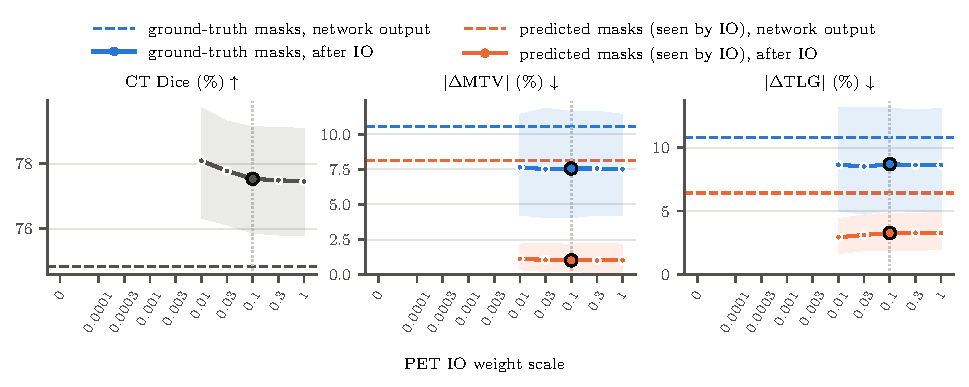
\includegraphics[width=\textwidth]{figures/tradeoff.pdf}
\caption{Effect of the PET loss weight in IO (test set): network trained without PET losses (T1) followed by IO with all PET weights scaled by the given factor (0: PET losses off; 1: the PET weights of network training). Dice over all 28 patients; lesion volume and uptake change on the predicted lesion masks that IO optimises (orange) and on the ground-truth masks used for evaluation (blue), over the 26 patients with lesions in both. Solid: after IO; dashed: network output before IO, the same for every factor. Outlined point and dotted line: operating point tuned on the validation set. Points: patient means; bands: 95\,\% patient-bootstrap confidence intervals.}
\label{fig:tradeoff}
\end{figure}
